\documentclass[border=8pt]{standalone}
\usepackage{fontspec}
\defaultfontfeatures{Ligatures=TeX}
\setmainfont{Palatino Linotype}
\setsansfont{Arial}
\usepackage{amsmath,amssymb}
\usepackage{tikz}
\usetikzlibrary{arrows.meta,positioning,calc,shapes.geometric,fit}
\definecolor{tksInk}{HTML}{1C1A16}
\definecolor{tksMuted}{HTML}{8A8378}
\definecolor{tksAccent}{HTML}{8C5A1F}
\definecolor{tksAfill}{HTML}{F6EEDD}
\definecolor{tksAedge}{HTML}{9A7328}
\definecolor{tksBfill}{HTML}{E6EDF5}
\definecolor{tksBedge}{HTML}{2F5B85}
\definecolor{tksCfill}{HTML}{F7E7E4}
\definecolor{tksCedge}{HTML}{95403A}
\definecolor{tksDfill}{HTML}{E4EFE6}
\definecolor{tksDedge}{HTML}{3A6B45}
\definecolor{tksEfill}{HTML}{F5DFDC}
\definecolor{tksEedge}{HTML}{A33B30}
\begin{document}
\centering
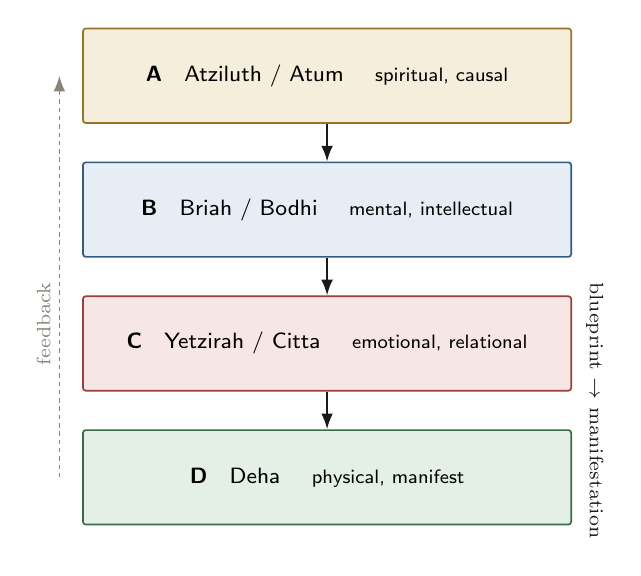
\begin{tikzpicture}[x=1mm, y=1mm, font=\sffamily\footnotesize,
  w/.style={rounded corners=1pt, minimum width=62mm, minimum height=12mm,
            draw, line width=0.6pt, align=center}]
  \node[w, fill=tksAfill, draw=tksAedge] (A) at (0,0)
    {\textbf{A} \; Atziluth / Atum \quad {\scriptsize spiritual, causal}};
  \node[w, fill=tksBfill, draw=tksBedge] (B) at (0,-17)
    {\textbf{B} \; Briah / Bodhi \quad {\scriptsize mental, intellectual}};
  \node[w, fill=tksCfill, draw=tksCedge] (C) at (0,-34)
    {\textbf{C} \; Yetzirah / Citta \quad {\scriptsize emotional, relational}};
  \node[w, fill=tksDfill, draw=tksDedge] (D) at (0,-51)
    {\textbf{D} \; Deha \quad {\scriptsize physical, manifest}};
  \foreach \a/\b in {A/B, B/C, C/D} {
    \draw[-{Latex[length=2mm]}, tksInk, line width=0.7pt] (\a) -- (\b);
  }
  \node[anchor=west, rotate=-90, font=\scriptsize, text=tksInk]
    at (34,-25) {blueprint $\rightarrow$ manifestation};
  \draw[-{Latex[length=2mm]}, tksMuted, line width=0.6pt,
        dash pattern=on 1.6pt off 1.4pt]
    (-34,-51) -- (-34,0);
  \node[anchor=east, rotate=90, font=\scriptsize, text=tksMuted]
    at (-36,-25) {feedback};
\end{tikzpicture}
\end{document}
